\documentclass[11pt, oneside]{article}	% use "amsart" instead of "article" for AMSLaTeX format
\usepackage{geometry}	
\usepackage{hyperref}
\geometry{a4paper}								% ... or letterpaper or a5paper or ... 
\usepackage{amsmath}
\usepackage{graphicx}							% Use pdf, png, jpg, or eps§ with pdflatex; use eps in DVI mode
\usepackage{bmpsize} 

% TeX will automatically convert eps --> pdf in pdflatex		
\usepackage{amssymb}
\usepackage{float}



\title{WEIBULL: $W_{pdf}$ maximum likelihood estimation, analysis}
\author{D. Palahnuk}
%\date{}										% Activate to display a given date or no date
\usepackage{comment}


\begin{document}
	\maketitle
	%\section{}
	%\subsection{}
	
\textbf{version 1.1: for repo release} \\

\textbf{For Weibull - We apply the MLE calculation:} \\


We start by assuming Weibull pdf that is ``Independent Identically Distributed'' which is usually designated as i.i.d. (or perhaps Markov depending on how you define or scope the analysis): 

$$
X = \left\{x_{1}, \ldots, x_{n}\right\}, \quad W{_{pdf}}(k, \lambda)
$$

$$
f(x ; \lambda, k)= \begin{cases}\frac{k}{\lambda}\left(\frac{x}{\lambda}\right)^{k-1} e^{-(x / \lambda)^{k}}, & x \geq 0 \\ 0, & x<0\end{cases}
$$


$$
L\left(\Theta \mid X \right)= L\left(x_{1}, \cdots x_{n} ; \gamma, \theta\right)=\prod_{i=1}^{n}(\gamma / \theta) x_{i}^{\gamma-1} \exp \left(-x_{i}^{\gamma} / \theta\right)
$$

Consider the maximum of $\log \left(L\left(\Theta \mid X \right)\right)$:\\

$$
\frac{\partial (\log L\left(\Theta \mid X \right))}{\partial \gamma}=0 
\quad and \quad
\frac{\partial (\log L\left(\Theta \mid X \right))}{\partial \theta}=0 
\quad and \quad 
$$\\

Solving the first order differentials:\\

$$
\frac{\partial \ln L}{\partial \gamma}=\frac{n}{\gamma}+\sum_{1}^{n} \ln x_{i}-\frac{1}{\theta} \sum_{1}^{n} x_{i}^{\gamma} \ln x_{i}=0
$$

$$
\frac{\partial \ln L}{\partial \theta}=-\frac{n}{\theta}+\frac{1}{\theta^{2}} \sum_{1}^{n} x_{i}^{\gamma} \quad=0
$$

On eliminating $\theta$ between these two equations and simplifying, we have
$$
\left[\frac{\sum_{1}^{n} x_{i}^{\gamma} \ln x_{i}}{\sum_{1}^{n} x_{i}^{\gamma}}-\frac{1}{\gamma}\right]=\frac{1}{n} \sum_{1}^{n} \ln x_{i},
$$


\noindent
We have to now solve the MLE for the best estimate of $\hat{\gamma}$. There is no analytic closed solution here for $\hat{\gamma}$, unfortunately. However, this can be solved by iteration, or trial and error. Once two values $\gamma_{1}$ and $\gamma_{2}$ have been found in an interval such that $\gamma_{1}<\gamma<\gamma_{2}$, end with a linear interpolation for $\hat{\gamma}$.\\




With $\hat{\gamma}$ thus determined, $\theta$ is estimated as

$$
\hat{\theta}=\sum_{1}^{n} x_{i}^{\hat{\gamma}} / n
$$
\noindent
Interestingly enough - this simply looks like the average of the $x_{i}$ at some power $\hat{\gamma}$.



\newpage
Example of WEIBULL PDF and Cpk in JMP\\ 

This data is what I like to refer to as ceiling (or floor) data - the data ranges up to a limit of 100 (or 0) percent. In this example it is a cell culture vial thaw viability distribution. Therefore, typically it won't be normally distributed. This type of distribution is often seen in the Biotech area - where we have a top 100 (or bottom 0) percent value as a ceiling.\\

We have a few choices: Transform it, do it non-parametrically, or use a suitable pdf. In this case the Weibull pdf is used since the shape is reasonable. Here we set the LSL (spec limit) to 80 percent, giving a calculated Ppk of 3.9. Therefore, the spec limit can be raised based on the process ANOVA for the viability in the vial thaw.\\ 

VIAL THAW Viability Distribution ANOVA: For the purposes of a non-Normal pdf in Cpk type capability analysis, here is the JMP restult. This follows from applying a Weibull pdf approach and is supported by MLE theory (roughly) derived above. 

\begin{figure}[H]
\centering
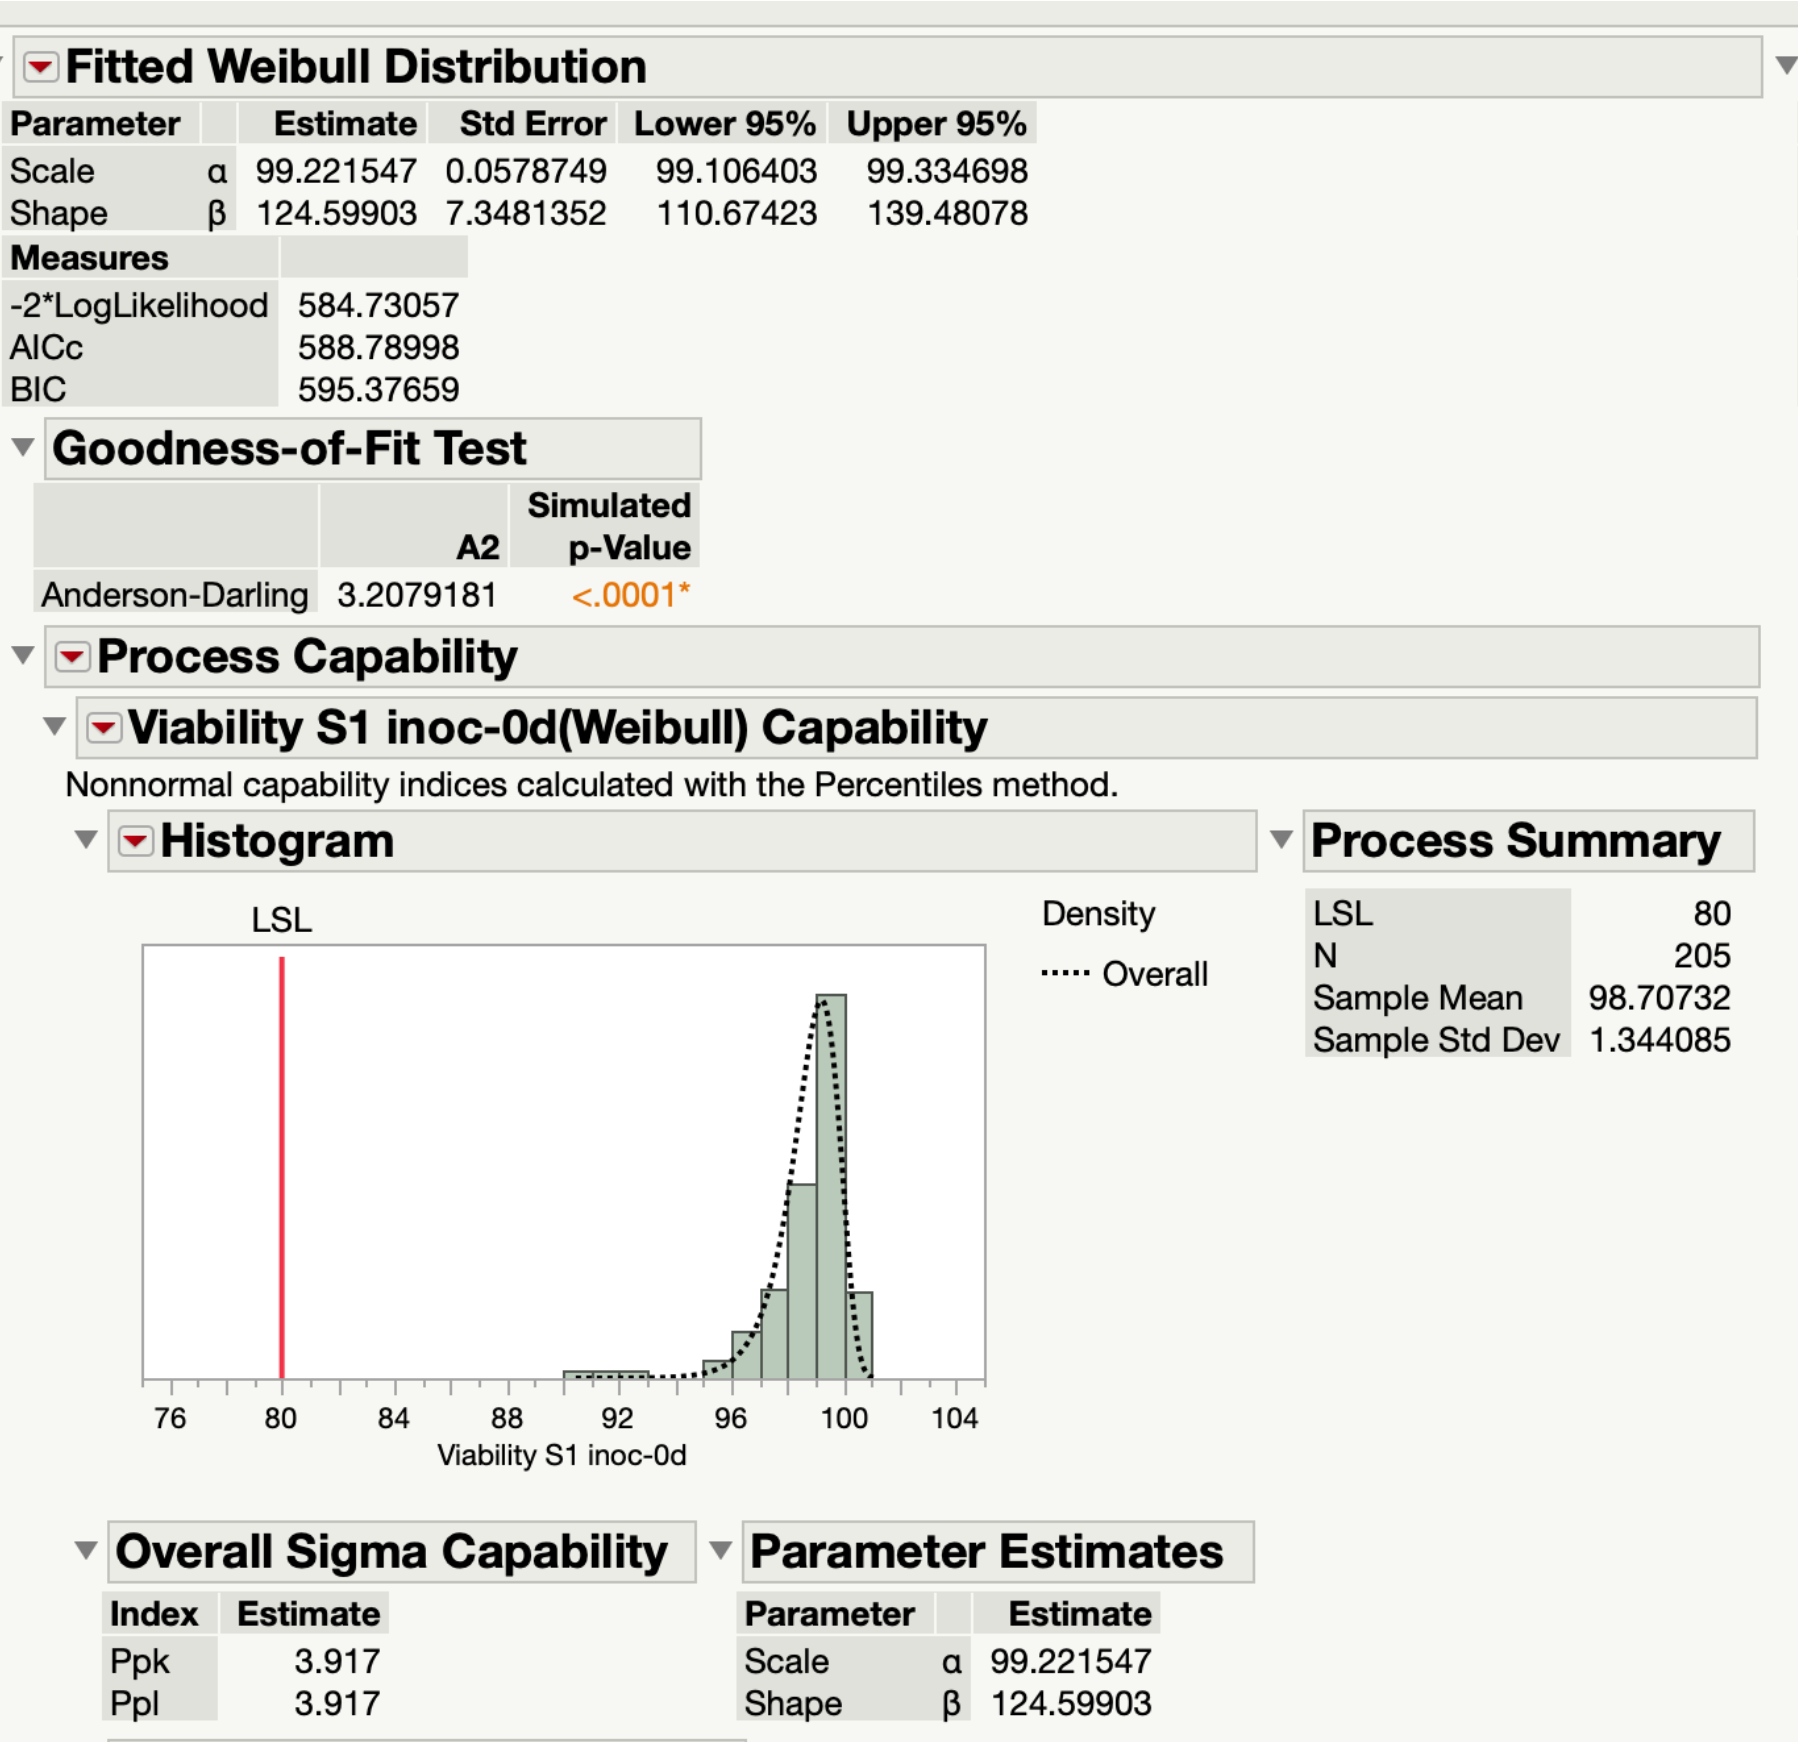
\includegraphics[scale=0.40]{Anova Weibull JS1 seed Example.png}
\end{figure}

\end{document}  



















